
%(BEGIN_QUESTION)
% Copyright 2009, Tony R. Kuphaldt, released under the Creative Commons Attribution License (v 1.0)
% This means you may do almost anything with this work of mine, so long as you give me proper credit

A butterfly-style control valve will be used to throttle combustion air flow to a large natural gas burner on an industrial furnace:

$$\includegraphics[width=15.5cm]{i01414x01.eps}$$

The pressure dropped across the burner is 8 ounces per square inch (8 oz/in$^{2}$).  At ``high fire'' (full air flow and full burner heat output) the blower outputs a static pressure of 35 "W.C. at a flow rate of 2,000 standard cubic feet per minute (2,000 SCFM).  The furnace pressure is controlled to equal atmospheric pressure at all times.

Given these conditions, what must the combustion air control valve's $C_{v}$ be at full-open in order to pass 2,000 SCFM to the burner?  Assume an ambient temperature of 45$^{o}$ F.  Also, calculate the approximate size of the valve (nominal pipe diameter, in inches) needed if the style is a 90-degree butterfly valve with an offset seat ($C_d = 29$).

\vskip 10pt

Use the following valve capacity equation for your calculations:

$$Q = 963 \> C_v \sqrt{{\Delta P (P_1 + P_2)} \over {G_g T}}$$

\noindent
Where,

$Q$ = Gas flow rate, in units of Standard Cubic Feet per Hour (SCFH)

$C_v$ = Valve capacity coefficient

$\Delta P$ = Pressure dropped across valve, pounds per square inch differential (PSID)

$P_1$ = Upstream valve pressure, pounds per square inch absolute (PSIA)

$P_2$ = Downstream valve pressure, pounds per square inch absolute (PSIA)

$G_g$ = Specific gravity of gas (Air at standard temperature and pressure = 1.0)

$T$ = Absolute temperature of gas in degrees Rankine ($^{o}$R)


\vfil

\underbar{file i01414}
\eject
%(END_QUESTION)





%(BEGIN_ANSWER)

This is a graded question -- no answers or hints given!

%(END_ANSWER)





%(BEGIN_NOTES)

This problem is really just a ``plug and play'' exercise where we solve for one variable in an equation by manipulating that equation and plugging in all the known values for the other variables in the proper units.  First, manipulating the flow equation to solve for $C_v$:

$$C_v = {Q \over 963 \sqrt{{\Delta P (P_1 + P_2)} \over {G_g T}}}$$

Next, we need to determine the values of all variables (other than $C_v$) to solve for $C_v$.  We are given some pressure values for this system, but it may be difficult to see exactly where they might fit into the equation ($\Delta P$, $P_1$, $P_2$).  One problem-solving technique we may apply here is to liken the air flow piping to an electric circuit, where the blower represents a voltage source, the valve represents a variable resistor, and the burner represents a fixed resistor.  Since the blower draws air from the surrounding atmosphere and the burner discharges air into the atmosphere, these points will be analogously represented in the schematic as {\it ground}:

$$\includegraphics[width=15.5cm]{i01414x02.eps}$$

$P_1$, $P_2$, and $\Delta P$ are equivalent to the battery voltage, ``Burner'' resistor voltage, and ``Valve'' voltage, respectively.  From the equivalent circuit, we can see that the ``valve's'' voltage drop must be the difference in pressure between the discharge of the blower and the inlet of the burner ($\Delta P = P_1 - P_2$).  Since the pressures for this equation are all specified in units of PSIA (PSI absolute), we must perform some unit conversions to translate the given pressure information into the proper units:

\begin{itemize}
\item{} $P_1$ = 35 "W.C.G = 1.2645 PSIG = 15.964 PSIA
\item{} $P_2$ = 8 oz./in$^{2}$ = 0.5 PSIG = 15.2 PSIA
\vskip 5pt
\item{} $\Delta P = P_1 - P_2$ = 15.964 PSIA $-$ 15.2 PSIA = 0.764 PSID
\end{itemize}

Since we know the gas in question is air, we may use a value of 1.0 for $G_f$.  The temperature will simply be 504.67 $^{o}$R (459.67 plus the temperature in degrees Fahrenheit).

\vskip 10pt

Finally, the given flow rate was specified in units of SCFM, and the equation is meant to use SCFH.  A simple multiplier of 60 converts the given figure of 2000 SCFM into 120000 SCFH.

\vskip 10pt

Now we are ready to ``plug and play'':

$$C_v = {120000 \over 963 \sqrt{{(0.764) (15.964 + 15.2)} \over {(1) (504.67)}}} = 573.53$$

\vskip 10pt

Calculating pipe diameter $d$ using the equation $C_d = {C_v \over d^2}$, we see that a 4.5 inch butterfly valve would be just about right for this application.

%INDEX% Final Control Elements, valve: sizing
%INDEX% Process: combustion furnace

%(END_NOTES)


